\documentclass[a4paper,titlepage]{book}
\usepackage[swapnames]{frontespizio}
\usepackage[italian]{babel}% tesi in italiano
\usepackage[
autostyle,italian=guillemets
% ... altre opzioni
]{csquotes}
\usepackage[
% ... opzioni
backend=biber
]{biblatex}
\usepackage{graphicx}
\usepackage{geometry}
\usepackage{float}
\usepackage{amsmath}
\usepackage[italian]{babel}
\usepackage{listings,xcolor}
\definecolor{javared}{rgb}{0.6,0,0} % for strings
\definecolor{javagreen}{rgb}{0.25,0.5,0.35} % comments
\definecolor{javapurple}{rgb}{0.5,0,0.35} % keywords
\definecolor{javadocblue}{rgb}{0.25,0.35,0.75} % javadoc

\begin{document}
\begin{frontespizio}
\Universita{Firenze}
\Logo[2.5cm]{}
\Dipartimento{Ingegneria Informatica}
\Corso{Ingegneria Informatica}
\Titolo{Development of methods for face mask detection}
\Candidato{Gemma~Vaggelli}
\Relatore{Prof.~Marco Bertini}
\NRelatore{Coordinatore}{}
\Annoaccademico{2019-2020}
\end{frontespizio}

\null\vspace{\stretch{1}}
\begin{flushright}
\textit{A mamma Cri}
\end{flushright}
\vspace{\stretch{2}}\null

\pagebreak

\section{Introduzione}


\section{Caratteristiche}


\subsection{Caratteristiche InsertionSort}

\subsection{Caratteristiche MergeSort}

\section{Prestazioni}
\subsection{Prestazioni InsertionSort}

\subsection{Prestazioni MergeSort}

\begin{equation*}
T(n) = \begin{cases}
\Theta(1) & \text{se $n$ = 1,}\\
2T(\frac{n}{2}) + \Theta(n) & \text{se $n$ $>$ 1.}
\end{cases}
\end{equation*}
L'equazione di T(n) in forma chiusa con notazione asintotica per il MergeSort è T(n) $= \Theta(n)$


\section{Documentazione}


\paragraph{Hardware}
I test sono stati eseguiti su un PC Desktop con sistema operativo Windows 10 Home a 64 bit, un processore Intel Core i5-7200U con 8Gb di RAM e Visual Studio Code come IDE.
 
\section{Prestazioni risultati sperimentali}
\subsection{Prestazioni risultati sperimentali caso Random}
\begin{center}
 \begin{tabular}{||c  c c||} 
 \hline
 Dim & Merge  & Ins \\ [0.5ex] 
\hline
0  & 0 & 0 \\
\hline
200 & 4 & 4 \\
\hline
\end{tabular}
\end{center}
\subsection{Prestazioni risultati sperimentali best case}
\begin{center}
 \begin{tabular}{||c  c c||} 
 \hline
 Dim & Merge  & Ins \\ [0.5ex] 
\hline 
0 & 0 & 0 \\
\hline
200 & 4 & 0 \\
\hline
\end{tabular}
\end{center}
\subsection{Prestazioni risultati sperimentali worst case}
\begin{center}
 \begin{tabular}{||c  c c||} 
 \hline
 Dim & Merge & Ins \\ [0.5ex] 
 \hline\hline
 \hline
0 & 0 & 0 \\
\hline
200 & 0 & 8 \\
\hline
5000 & 40 & 6168 \\ 
 \hline
\end{tabular}
\end{center}
\subsection{Grafici}
\begin{figure}[H]
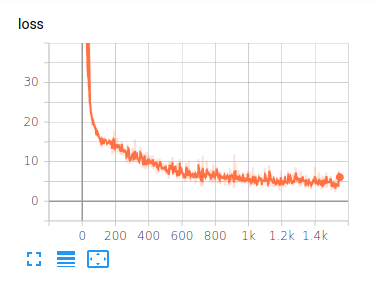
\includegraphics[width=\textwidth]{loss.png}
\caption{Ordinamento di array causale}
\end{figure}
\section{Analisi risultati sperimentali}
\subsection{Analisi risultati sperimentali InsertionSort} 

\subsection{Analisi risultati sperimentali MergeSort}


\section{Conclusione}




\end{document}